\documentclass[11pt]{article}

\usepackage[letterpaper,margin=0.75in]{geometry}
\usepackage{booktabs}
\usepackage{graphicx}
\usepackage{listings}
\usepackage{hyperref}

\setlength{\parindent}{1.4em}

\begin{document}

\lstset{
  language=Python,
  basicstyle=\small,          % print whole listing small
  keywordstyle=\bfseries,
  identifierstyle=,           % nothing happens
  commentstyle=,              % white comments
  stringstyle=\ttfamily,      % typewriter type for strings
  showstringspaces=false,     % no special string spaces
  numbers=left,
  numberstyle=\tiny,
  numbersep=5pt,
  frame=tb,
}

\newenvironment{absolutelynopagebreak}
  {\par\nobreak\vfil\penalty0\vfilneg
   \vtop\bgroup}
  {\par\xdef\tpd{\the\prevdepth}\egroup
   \prevdepth=\tpd}

\title{Network Simulation}

\author{Cody Heffner}

\date{19 Mar. 2015}

\maketitle

\section{Preface}

This report details the experiment I ran and the results obtained as specified by the Congestion Control Lab in the BYU CS 460 class taught by Dr. Zappala. The project specifications can be found \href{http://cs460.byu.edu/winter-2015/labs/congestion-control-part-2}{here}.

The experiment requires heavy use of a network simulator to test different network scenarios. The network simulator I used is Dr. Zappala's \href{https://github.com/zappala/bene}{Bene}, written in Python. All my simulation examples shown will be tailored towards use for that simulator.

\section{Summary}

The goal of this lab was to implement congestion control in my implementation of TCP. This includes implementing TCP slow start and TCP additive increase, multiplicative decrease, as well as a fast-retransmit function. This portion of the lab specifically tests congestion when there is more than one flow incoming to the same node.

In every experiment other than the final one (\emph{Advanced Experiment: Competing Round Trip Time}), I created a network consisting of two nodes and one bi-directional link with a link bandwidth of 10 Mbps, 10 ms propagation delay, and a queue size of 100 packets (100,000 bytes). The test file was of size 1 MB.

\section{Basic Experiment: One Flow}

This experiment's purpose was to establish a base case and teach us what a single flow looks like. The following three figures respectively show the sequence graph, a graph of the receiver's rate over time during the download, and a scatter plot of the queue during the download.

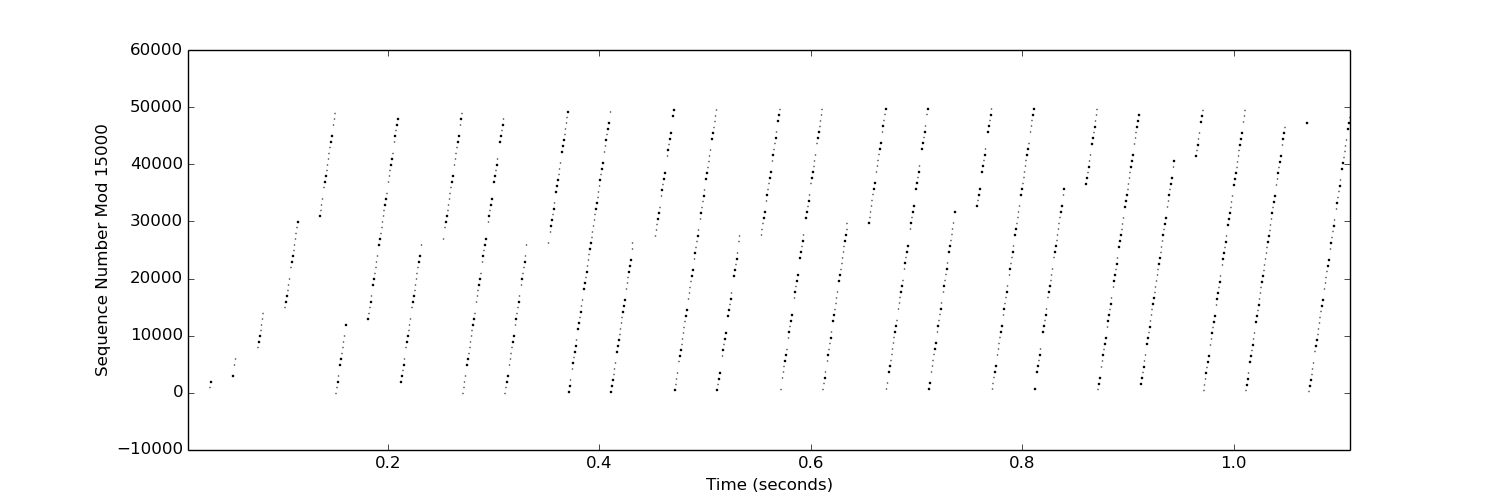
\includegraphics[width=17cm]{outputs/oneflow/converted_oneflow.txt_sequence.png}
\emph{Figure 1.1: Sequence Graph of One Flow}
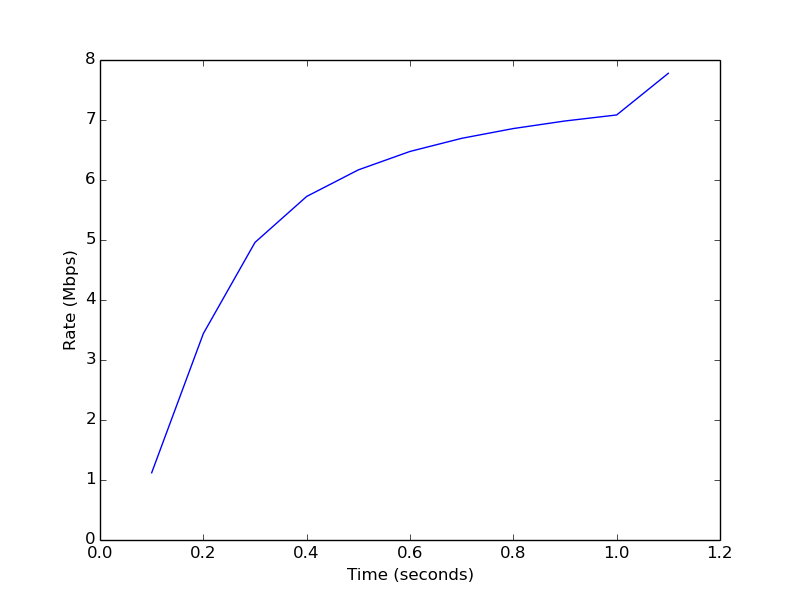
\includegraphics[width=17cm]{outputs/oneflow/converted_oneflow.txt_rate.png}
\emph{Figure 1.1: Rate Graph of One Flow}
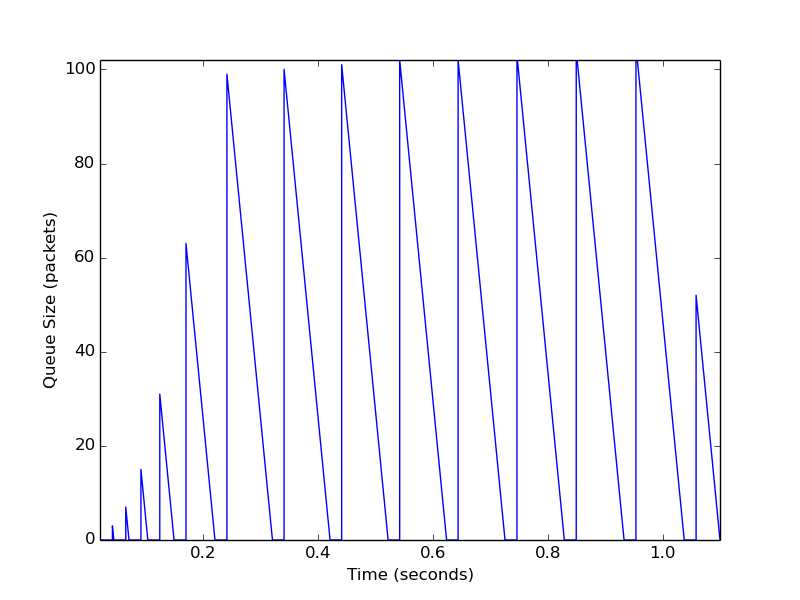
\includegraphics[width=17cm]{outputs/oneflow/converted_queue_oneflow.txt_queue.png}
\emph{Figure 1.1: Queue Graph of One Flow}

% \vspace{5mm}
% \begin{absolutelynopagebreak}
% \begin{lstlisting}
% def loss_event(self):
%     self.threshold = max(self.window/2, self.mss)
%     self.window = 1 * self.mss

% # slow start & AI
% def increase_window(self, amount):
%     # loss event check
%     self.duplicates += 1
%     if amount == 0 and self.duplicates >= 4:
%         self.loss_event()
%     else:
%         self.duplicates = 0

%         # AI
%         if amount + self.window >= self.threshold:
%             self.window += (self.mss * amount / self.window)
%             self.threshold = self.window
%         # slow start
%         else:
%             self.window += amount
% \end{lstlisting}
% \end{absolutelynopagebreak}
% \vspace{5mm}

% \section{Tests}

% Slow Start: To test slow start, I transferred a small file that transferred entirely within the range of slow start. In the following graph, the reader should notice that each set of segments doubles in size. 

% 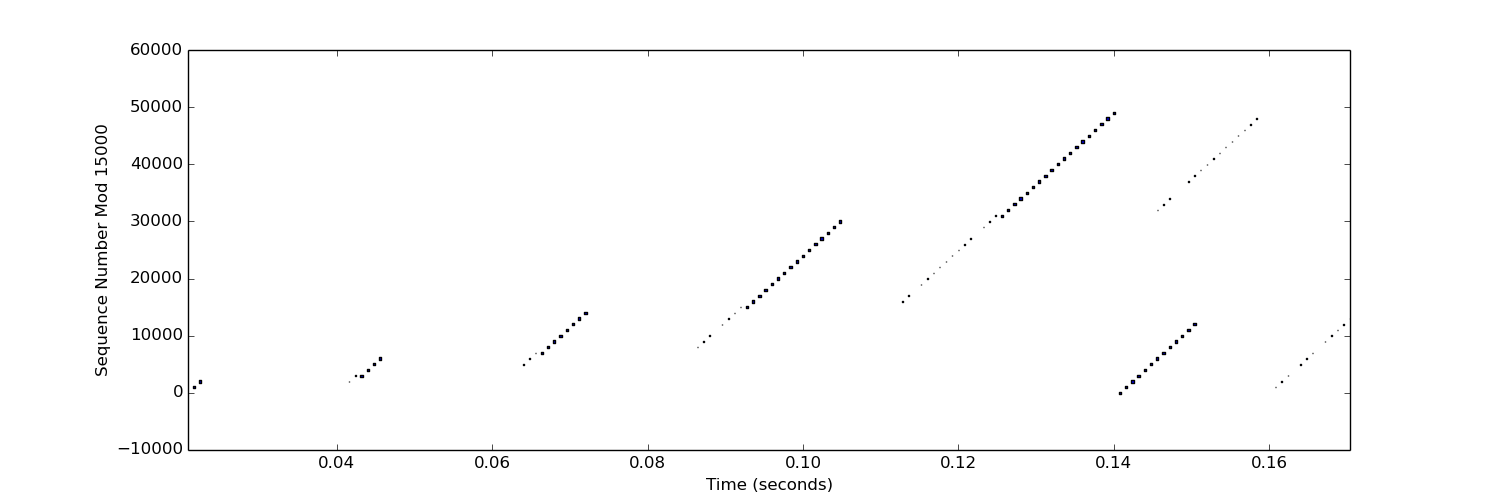
\includegraphics[width=17cm]{outputs/converted_output1.png}

% Additive Increase: To test additive increase, I transferred a larger file with a threshold of 16,000 bytes, i.e., 16 segments.  The reader can observe in the following graph that each set of segments doubles in size, like in the previous graph, until the sender sends 16 segments. The next set is 17 segments in size, and the final set is also 17 segments in size, which concluded the file transfer.

% 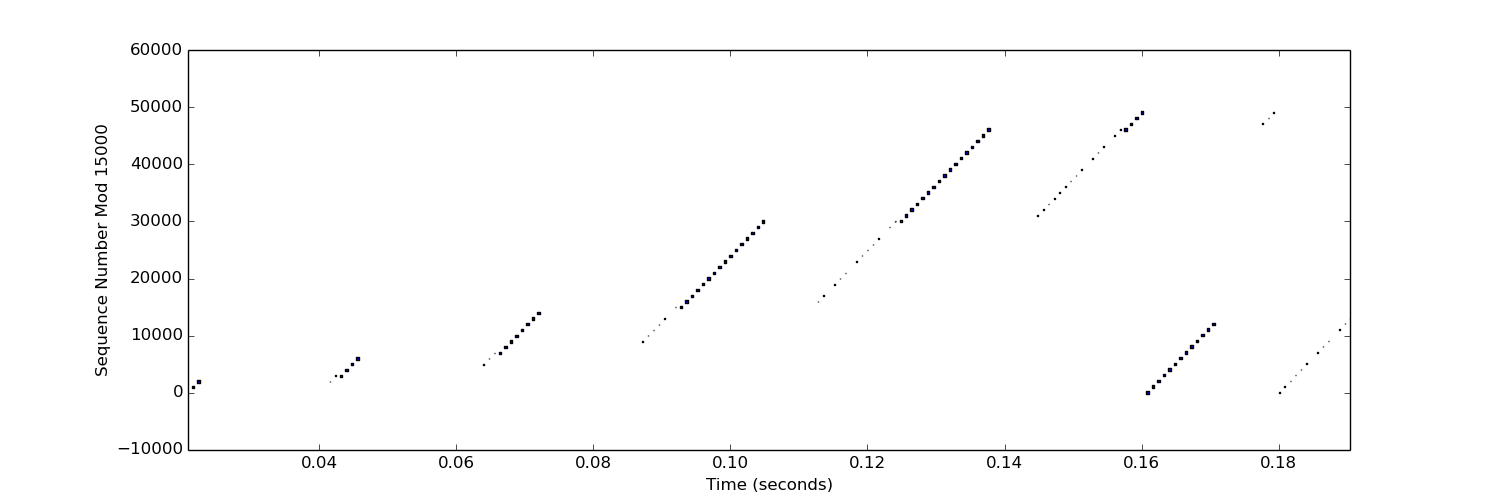
\includegraphics[width=17cm]{outputs/converted_output2.png}

\end{document}
